\documentclass[aspectratio=169,11pt,hyperref={colorlinks=true}]{beamer}
% https://github.com/zr-tex8r/BXcjkjatype/blob/master/README-ja.md
\usepackage[whole]{bxcjkjatype}
\usetheme{boxes}
\setbeamertemplate{navigation symbols}{}
\definecolor{suse}{RGB}{2, 211, 95}
\definecolor{susedark}{RGB}{13, 44, 64}
\definecolor{linkcolor}{RGB}{13, 44, 255}
\setbeamercolor{titlelike}{fg=suse}
\setbeamercolor{structure}{fg=suse}
\hypersetup{colorlinks,urlcolor=linkcolor}
\setbeamertemplate{footline}[frame number]
% Inserting graphics
\usepackage{graphicx}
% Side-by-side figures, etc
\usepackage{subfigure}
% Code snippits
\usepackage{listings}
% Color stuff
\usepackage{color}
% underline
\usepackage{soul}
% calc
\usepackage{calc}

\usepackage{amsmath}
\usepackage{tikz}
\newcommand\RBox[1]{%
  \tikz\node[draw,rounded corners,align=center,] {#1};%
}
\usepackage{hyperref}
%\usecolortheme{buzz}
%\usecolortheme{wolverine}
%\usetheme{Boadilla}
\usepackage[T1]{fontenc}
%\usepackage{fontspec}
%\usepackage[expert, deluxe]{otf}

\definecolor{mygreen}{rgb}{0,0.6,0}
\definecolor{mygray}{rgb}{0.5,0.5,0.5}
\definecolor{mymauve}{rgb}{0.58,0,0.82}


%\usepackage{CJK}
%\pdfmapline{=genshingothic@Unicode@ <genshingothic.ttf}
% bxcjkjatype
%\setgothicfont[<ID>]{<フォントファイル名>}
%\setgothicfont{/Users/foo/Library/Fonts/genshingothic.ttf}
%\setgothicfont{/Users/foo/Library/Fonts/NotoSansCJKjp-Regular.otf}
%\setgothicfont{/Users/foo/Downloads/genshingothic-20150607/GenShinGothic-P-Normal.ttf}
%\setgothicfont{/Users/foo/Downloads/genshingothic-20150607/GenShinGothic-Regular.ttf}
%\setgothicfont{hiragino.ttc}
\setgothicfont{mplus-1p-regular.ttf}
\setCJKfamilydefault{\gtdefault}
%\setCJKfamilydefault{\mcdefault}
%\CJKforce{abcdefghijklmnopqrstuvwxyzABCDEFGHIJKLMNOPQRSTUVWXYZ}


\lstset{%
  backgroundcolor=\color{white},   % choose the background color; you must add \usepackage{color} or \usepackage{xcolor}
  breakatwhitespace=false,         % sets if automatic breaks should only happen at whitespace
  breaklines=true,                 % sets automatic line breaking
  captionpos=b,                    % sets the caption-position to bottom
  commentstyle=\color{suse},  % comment style
  extendedchars=true,              % lets you use non-ASCII characters; for 8-bits encodings only, does not work with UTF-8
  keepspaces=true,                 % keeps spaces in text, useful for keeping indentation of code (possibly needs columns=flexible)
  keywordstyle=\color{blue},       % keyword style
%  otherkeywords={*,...},           % if you want to add more keywords to the set
  numbersep=5pt,                   % how far the line-numbers are from the code
  numberstyle=\tiny\color{mygray}, % the style that is used for the line-numbers
  rulecolor=\color{white},         % if not set, the frame-color may be changed on line-breaks within not-black text (e.g. comments (green here))
  showspaces=false,                % show spaces everywhere adding particular underscores; it overrides 'showstringspaces'
  showstringspaces=false,          % underline spaces within strings only
  showtabs=false,                  % show tabs within strings adding particular underscores
  stringstyle=\color{suse},   % string literal style
}

\setbeamerfont{caption}{series=\normalfont,size=\fontsize{6}{8}}
%\setbeamerfont{caption}{series=\normalfont,size=\large}
\setbeamertemplate{caption}{\raggedright\insertcaption\par}

\setlength{\abovecaptionskip}{0pt}
\setlength{\floatsep}{0pt}

%%%%%%%%%%%%%%%%%%%%%%%%%%%%%%%%%%%%%%%%%%%%%%%%%%%%%%%%%%%%%%%%%%%%%

\author[Masayuki Igawa]{%
    \texorpdfstring{%
        \begin{columns}
        \column{.7\linewidth}
            \centering
            Masayuki Igawa: \href{mailto:masayuki@igawa.io}{masayuki@igawa.io}\\
            \texttt{masayukig on
              \href{https://freenode.net/}{Freenode},
              \href{https://github.com/masayukig}{GitHub},
              \href{https://twitter.com/masayukig}{Twitter},
              \href{https://www.linkedin.com/in/masayukig/}{LinkedIn}}
        \end{columns}
        }
    {Masayuki Igawa}
}
\date{\href{https://events.opensuse.org/conferences/summitasia19/program/proposals/2762}{@Room 201, 13:45-14:30, October 6, 2019}}
\def\place#1{\def\@place{#1}}
\place{\href{https://events.opensuse.org/conferences/summitasia19}{@openSUSE.Asia Summit 2019}}

%\vspace*{30pt}
\title[oss-development-inside-story
  \hspace{4em}\insertframenumber/\inserttotalframenumber]{How to Participate Open Source development\\
  - Open Source development tooling and community in the upstream -}

\setbeamercolor{background canvas}{bg=white}
\setbeamercolor{titlelike}{fg=black}
\setbeamercolor{structure}{fg=black}
\setbeamercolor{normal text}{fg=black}

\begin{document}
\setbeamertemplate{background canvas}{
\includegraphics[width=\paperwidth,height=\paperheight]{images/opensuse_base.png}}
{%
\setbeamertemplate{background canvas}{
\includegraphics[width=\paperwidth,height=\paperheight]{images/opensuse_preface.png}}
\setbeamertemplate{footline}{}
\setbeamercolor{background canvas}{bg=white}
\begin{frame}[noframenumbering]
  \hypersetup{colorlinks,urlcolor=susedark}
  \setbeamercolor{author}{fg=black}
  \setbeamercolor{date}{fg=black}
  \setbeamercolor{place}{fg=black}
  \titlepage{}
  \centering
  \@place \par
  \href{https://github.com/masayukig/oss-development-inside-story}{https://github.com/masayukig/oss-development-inside-story}
  %\vspace{1em}
  \begin{flushright}
    \tiny\href{https://creativecommons.org/licenses/by/4.0/}{This work
      is licensed under a Creative Commons Attribution 4.0
      International License.}~
\includegraphics[scale=0.3]{images/cc_by.png}
  \end{flushright}
\end{frame}
}

\section{Agenda}
\begin{frame}
  \frametitle{Agenda}
  \begin{enumerate}
    \item About me
    \item Today's Goal
    \item Open Source Communities
    \item OpenStack as an example
    \item True Stories
    \item How to Participate
    \item Summary
  \end{enumerate}
\end{frame}

\section{DISCLAIMER}
\begin{frame}
  \frametitle{DISCLAIMER}
  \Huge{\bf{These slides are my own opinion}}
\end{frame}

\section{About me}
\begin{frame}
  \frametitle{About me}
  \begin{itemize}
    \item Company:1998.4-2015.12 Traditional IT company in Japan,\\
      2016.1-2017.3 HPE -> 2017.3- SUSE -> 2019(\href{https://www.suse.com/c/further-independence-for-suse/}{\scriptsize{``Further Independence for SUSE''}})
      \begin{itemize}
        \item SUSE OpenStack Cloud Team
      \end{itemize}
    \item Job: Senior Software Engineer/Open Source Programmer
      \begin{itemize}
        \begin{scriptsize}
        \item \href{https://www.openstack.org/}{OpenStack}
          \href{https://wiki.openstack.org/wiki/QA}{QA} Up/Downstream development, Core Reviewer
        \item[]
          (\href{https://docs.openstack.org/developer/tempest/}{Tempest},
          \href{http://status.openstack.org/openstack-health/}{OpenStack-Health},
          \href{https://docs.openstack.org/developer/subunit2sql/}{Subunit2SQL},
          \href{https://docs.openstack.org/developer/stackviz/}{Stackviz},etc.),
          \href{https://github.com/mtreinish/stestr}{stestr}
        \item
          \href{http://stackalytics.com/?user_id=igawa&release=all&metric=all}{stackalytics.com/?user\_id=igawa},
          \href{https://github.com/masayukig}{github.com/masayukig}
        \end{scriptsize}
      \end{itemize}
    \item Books 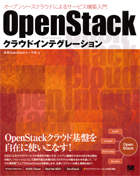
\includegraphics[scale=0.2]{images/OpenStack_Integration_book.png}~
\includegraphics[scale=0.2]{images/InfraCI_book.png}
      \begin{itemize}
      \item \href{https://www.amazon.co.jp/dp/4798139785/}{\scriptsize{OpenStack
        Cloud Integration (Japanese book)}} (one of the authors)
      \item \href{https://www.amazon.co.jp/dp/4798155128/}{\scriptsize{Infra CI
        Pragmatic Guide - Ansible/GitLab (Japanese book)}} (as a reviewer)
      \end{itemize}
    \item Hobby: Bike(BMC SLR02), Clouds(OpenStack...), Diet(Low-carb), etc.
  \end{itemize}
  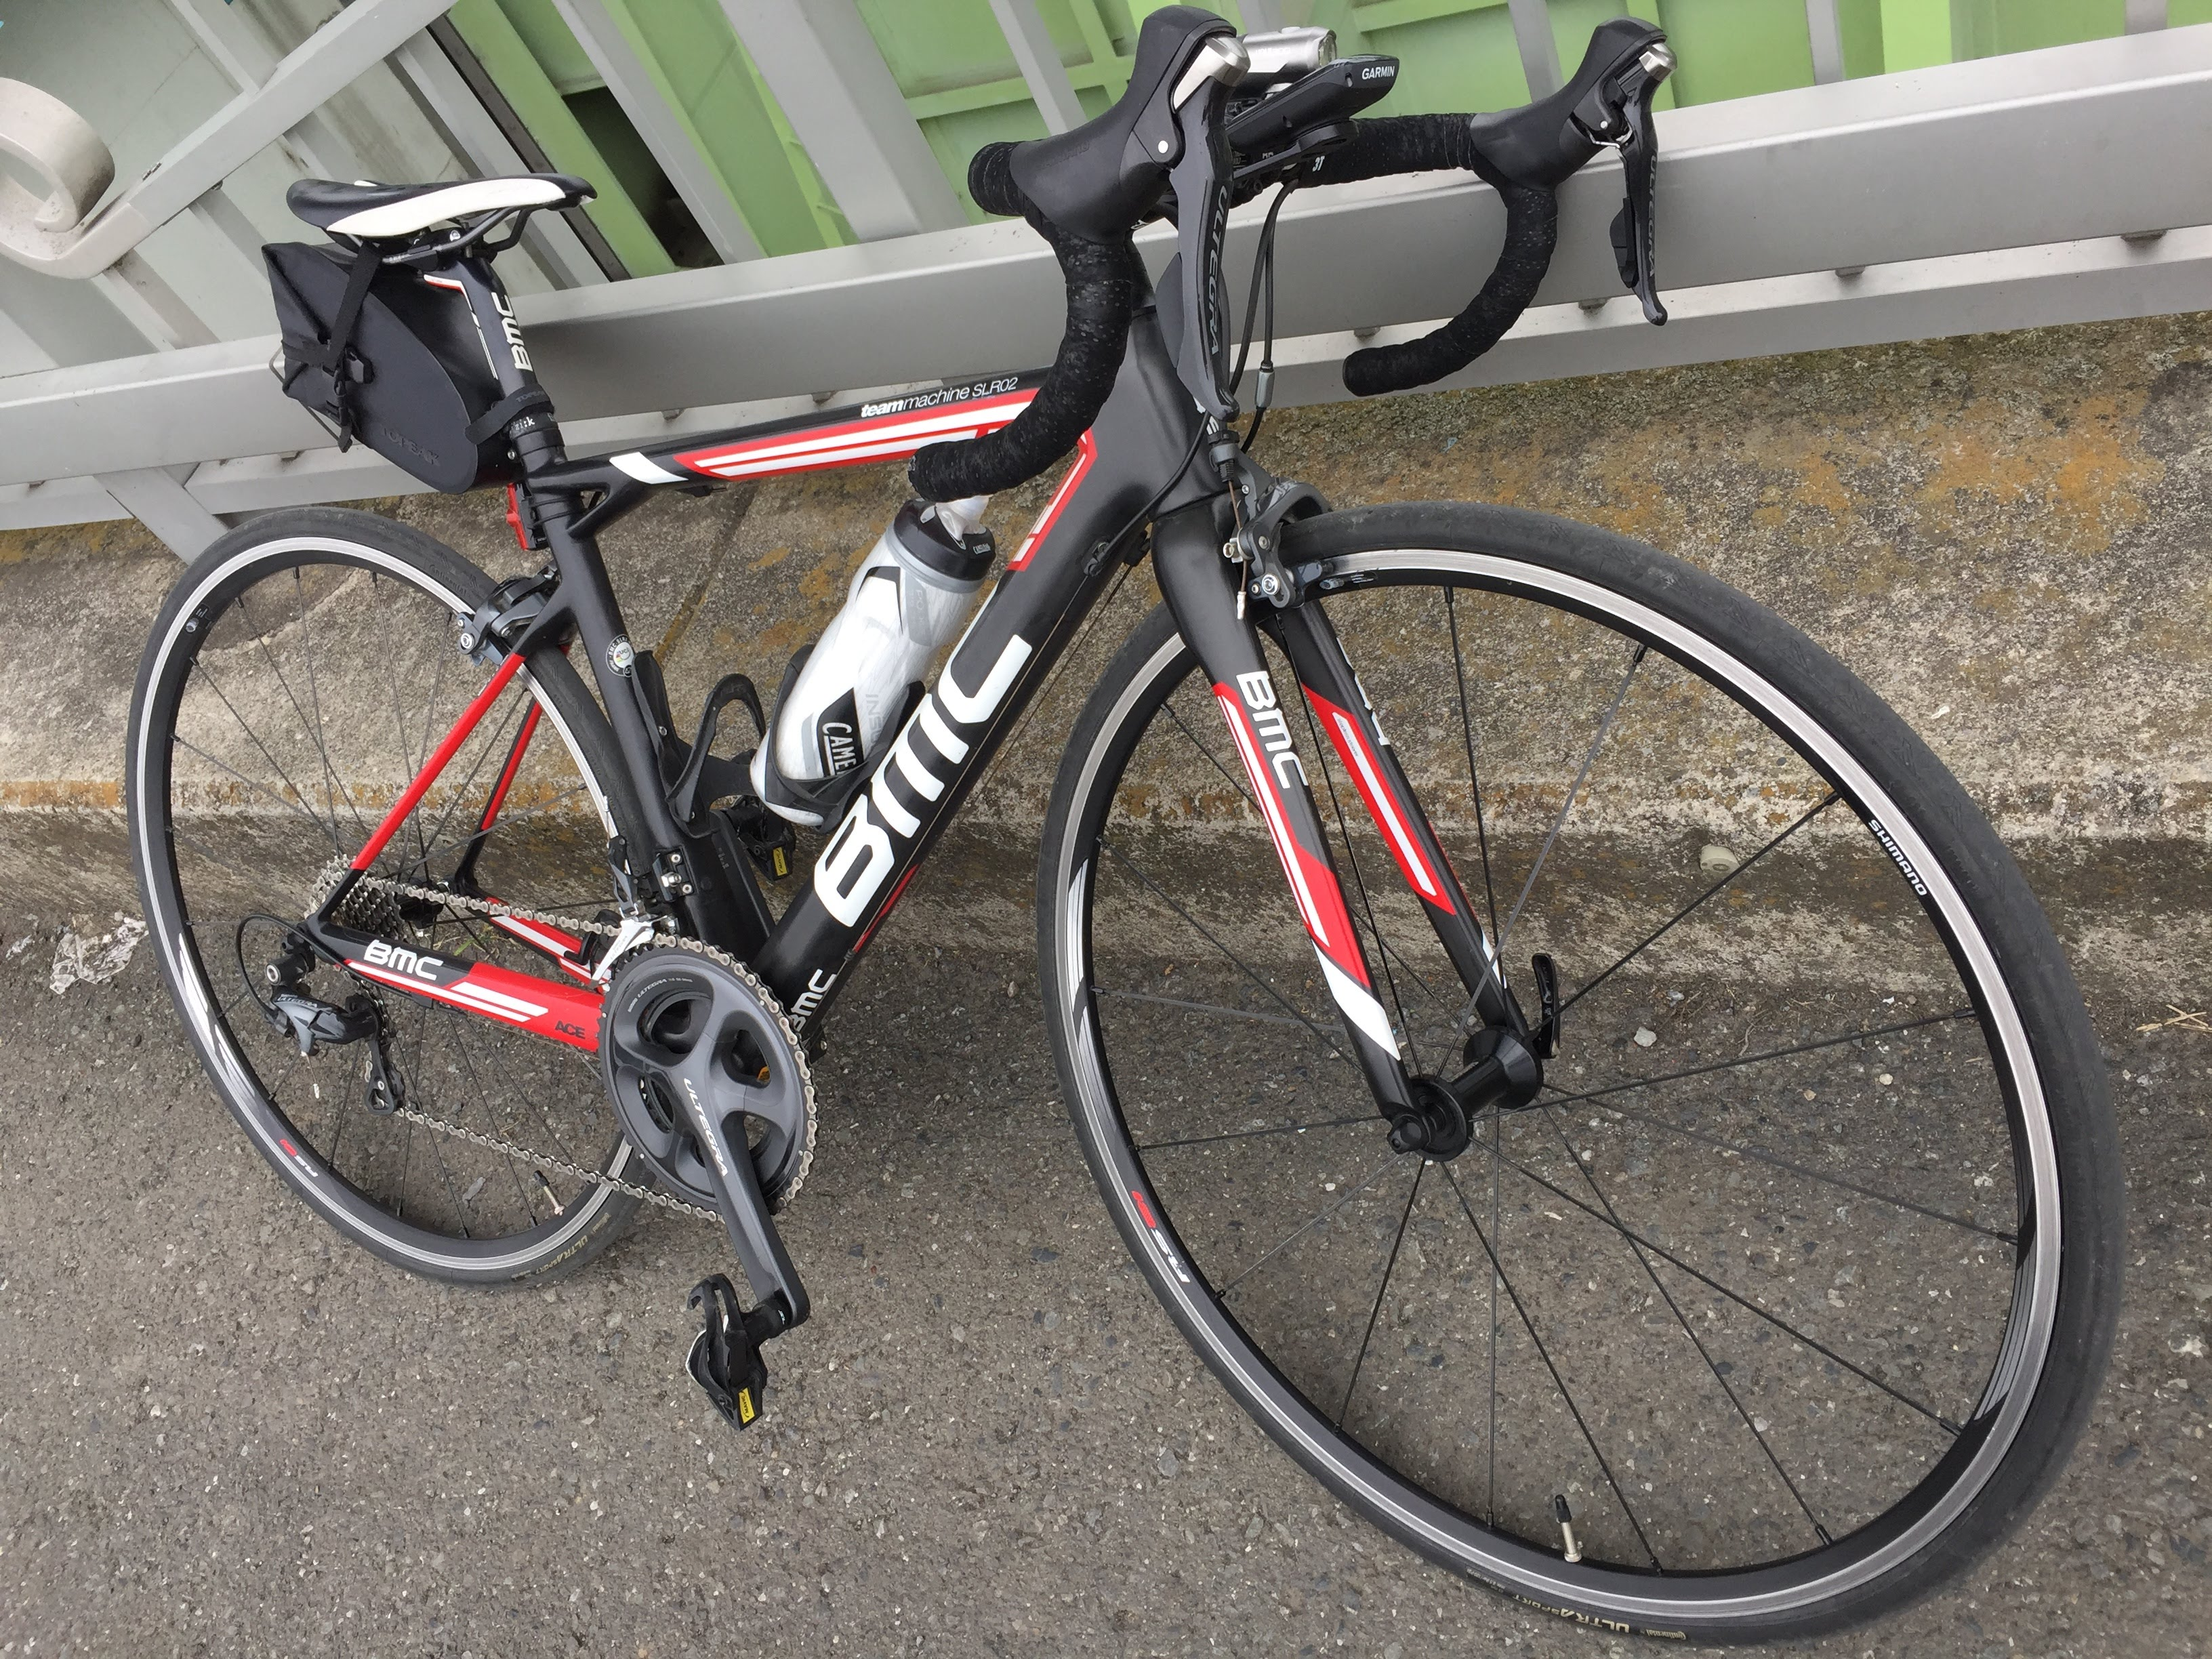
\includegraphics[height=20mm]{images/my-bike.jpg}~
  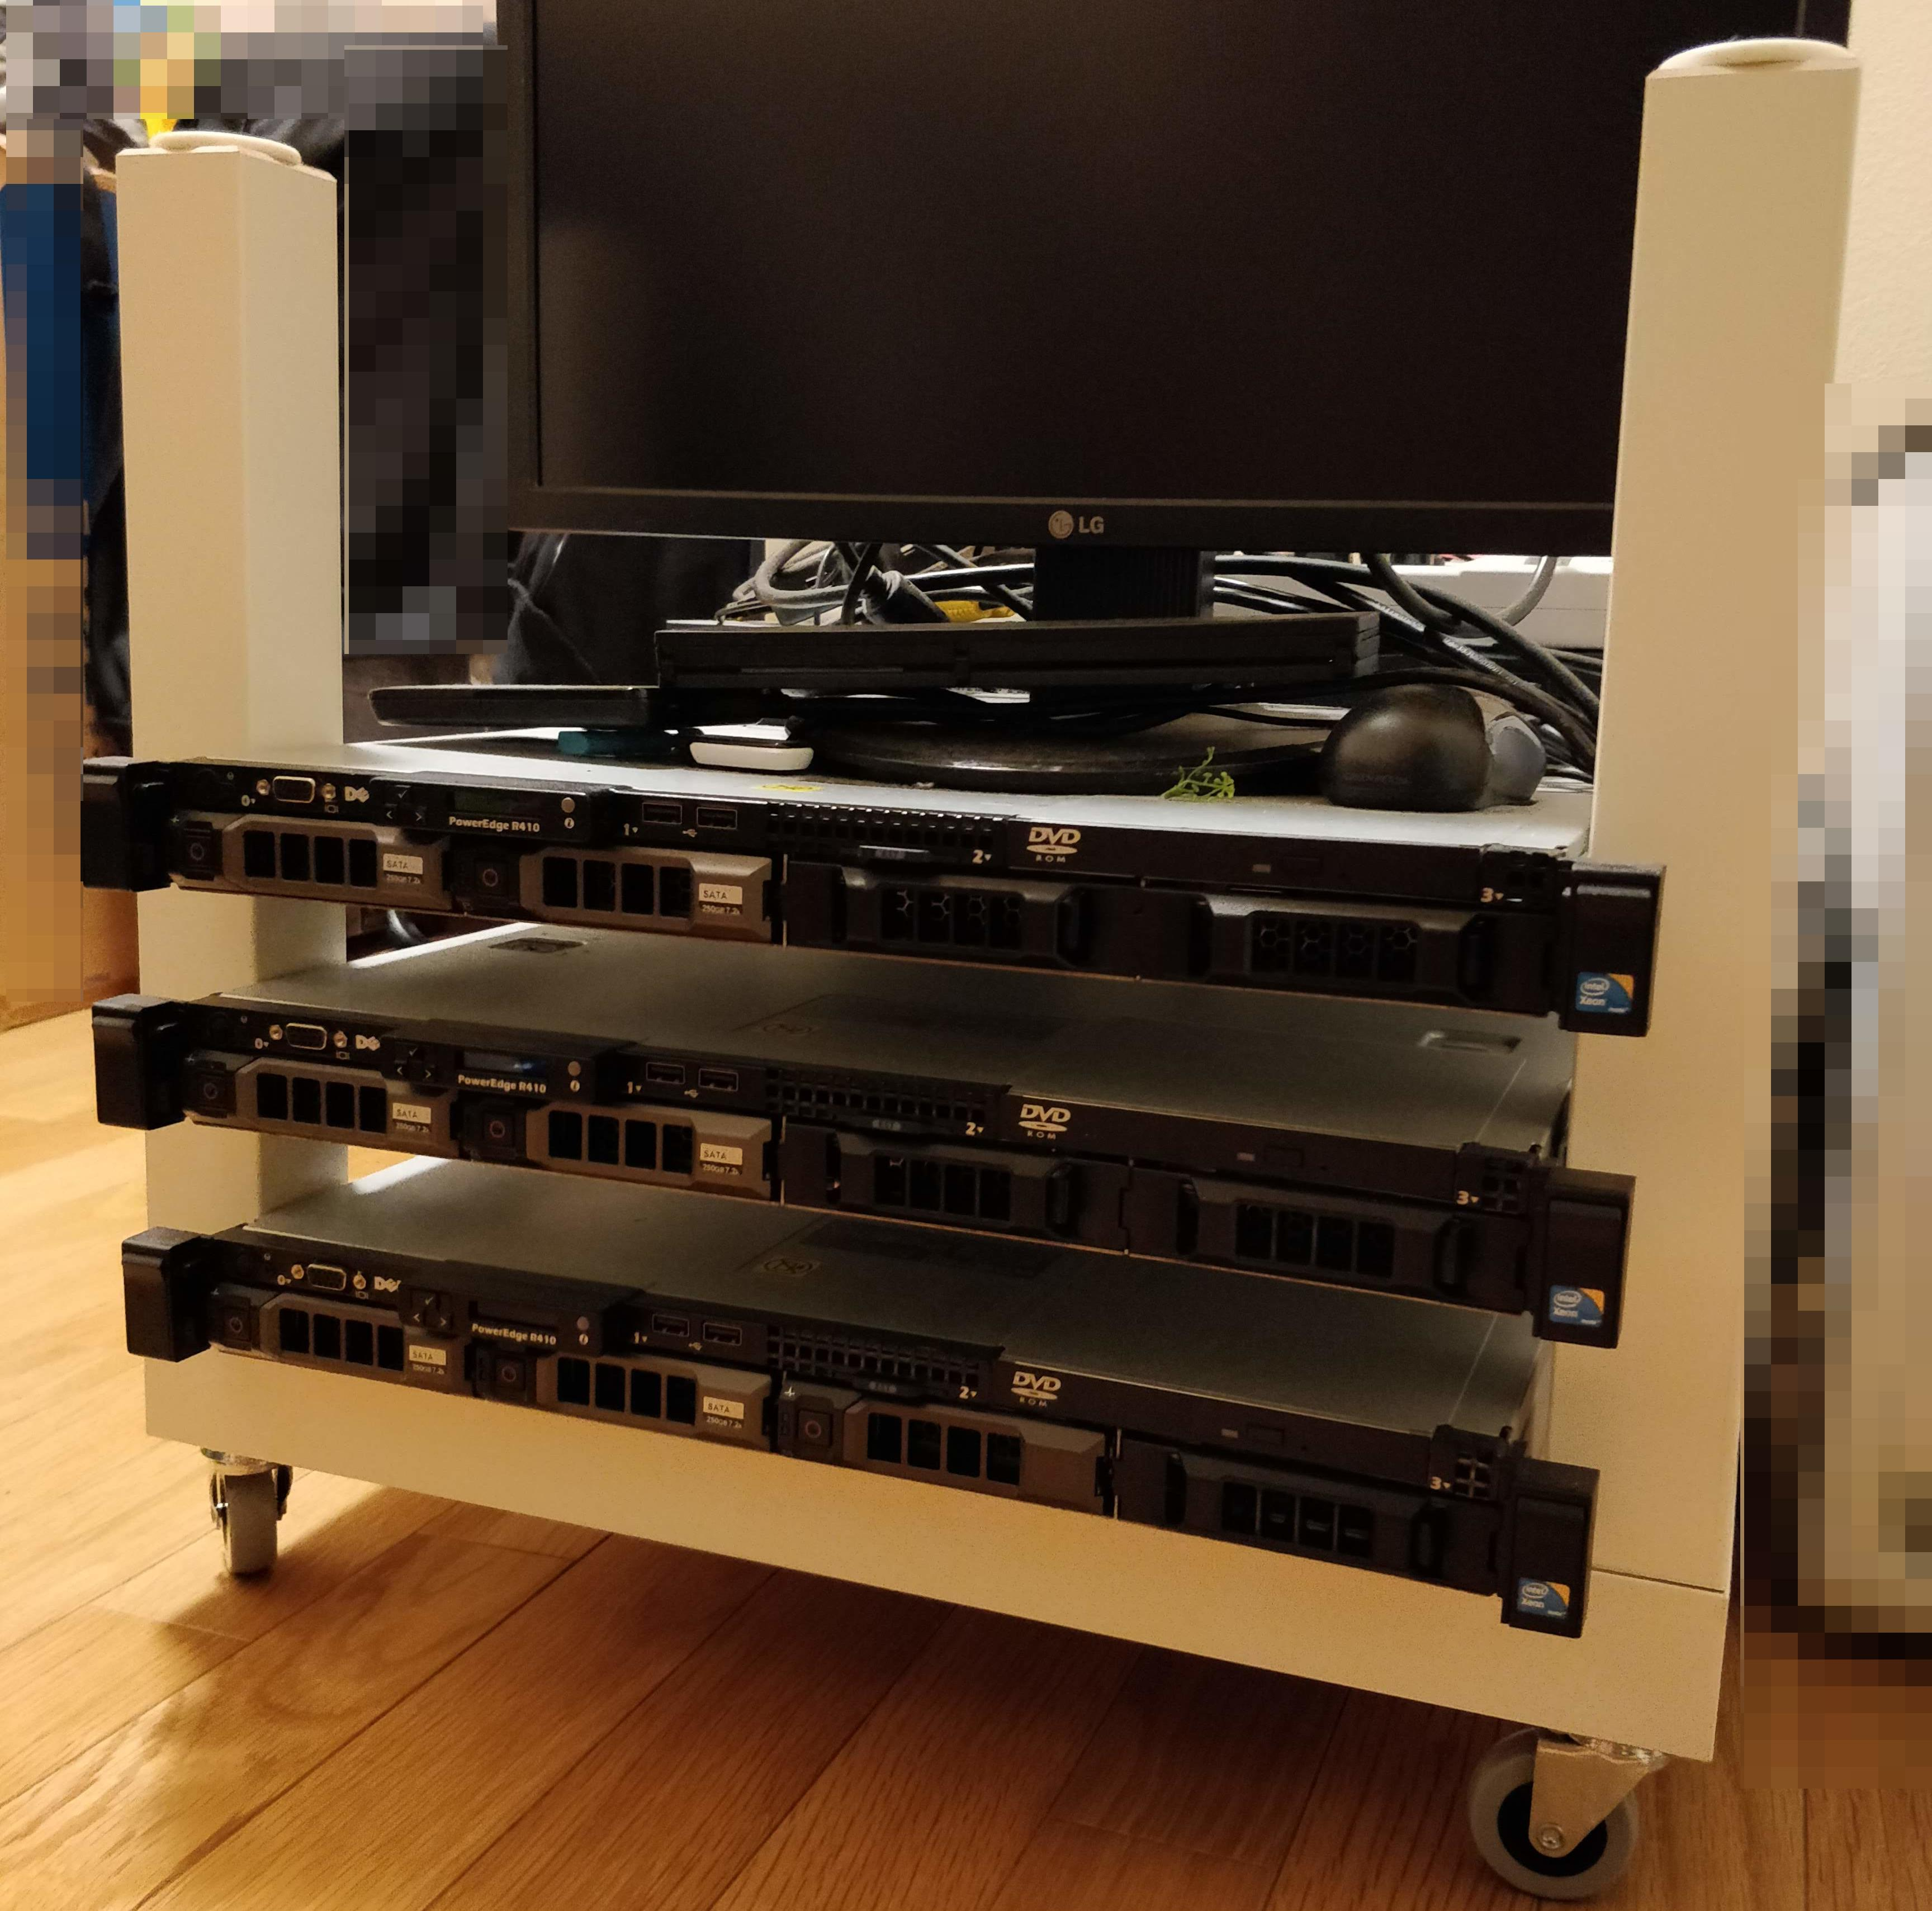
\includegraphics[height=20mm]{images/server_front.jpg}~
  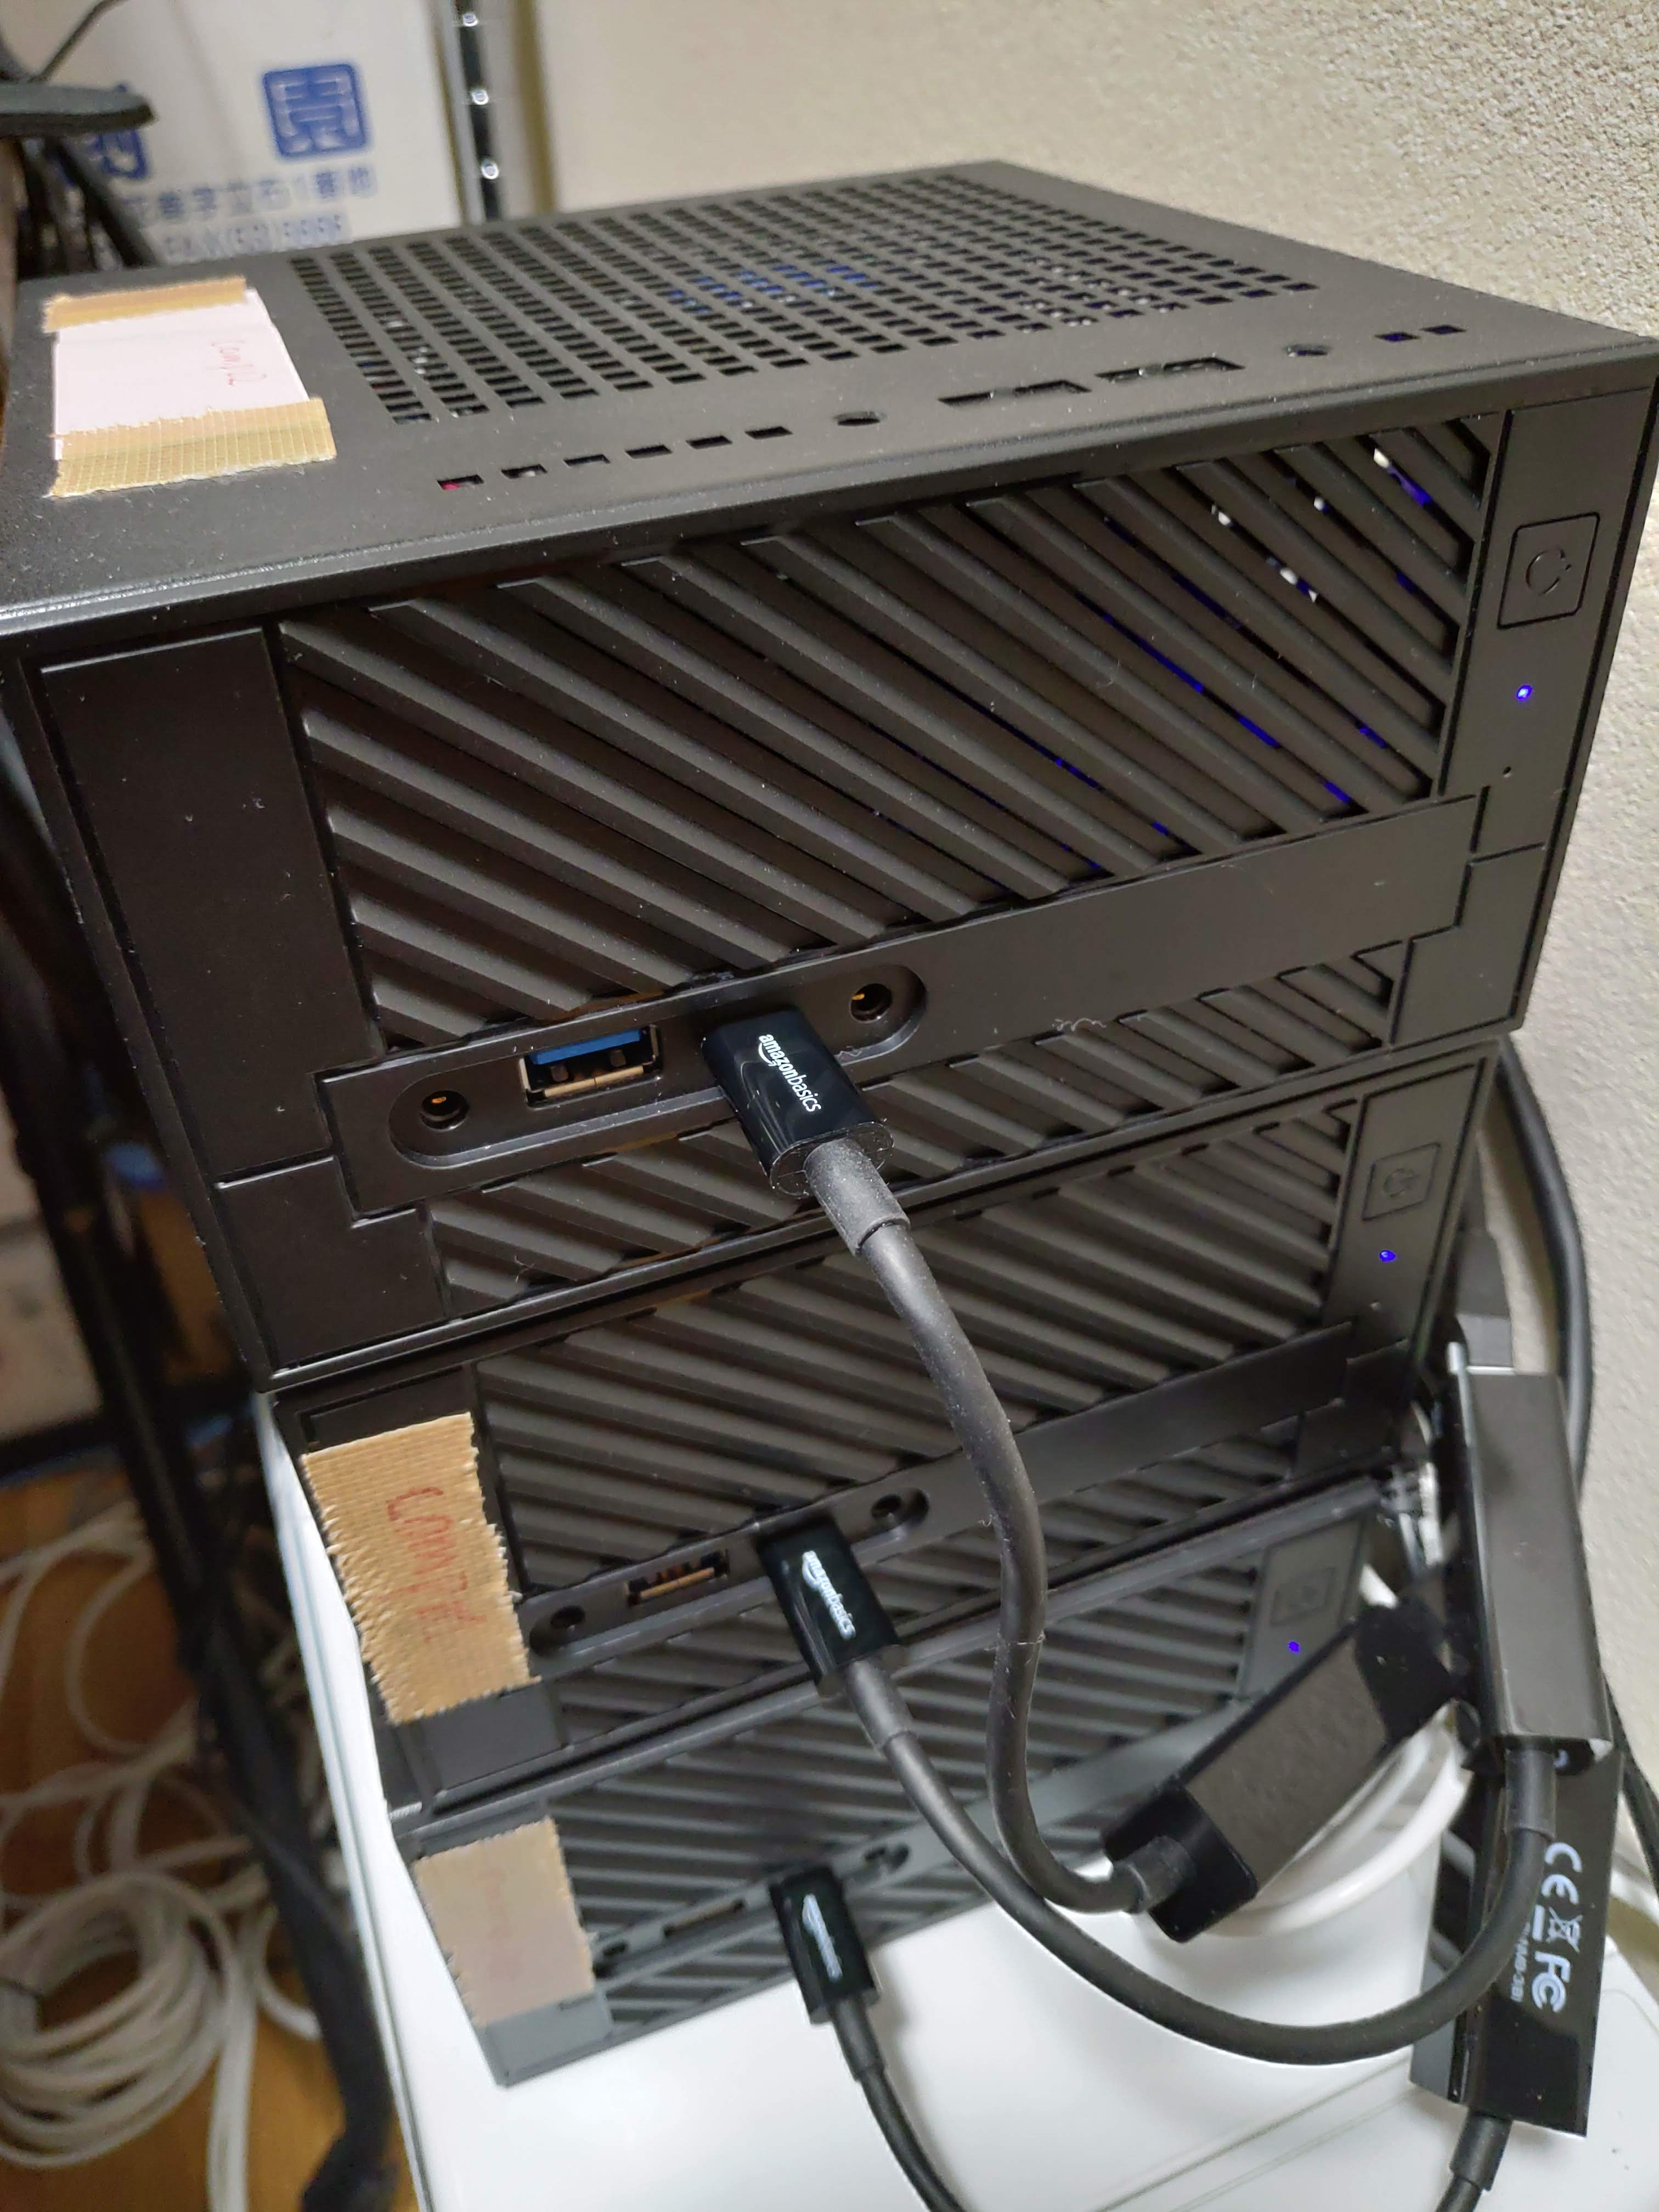
\includegraphics[height=20mm]{images/my-small-server.jpg}~
  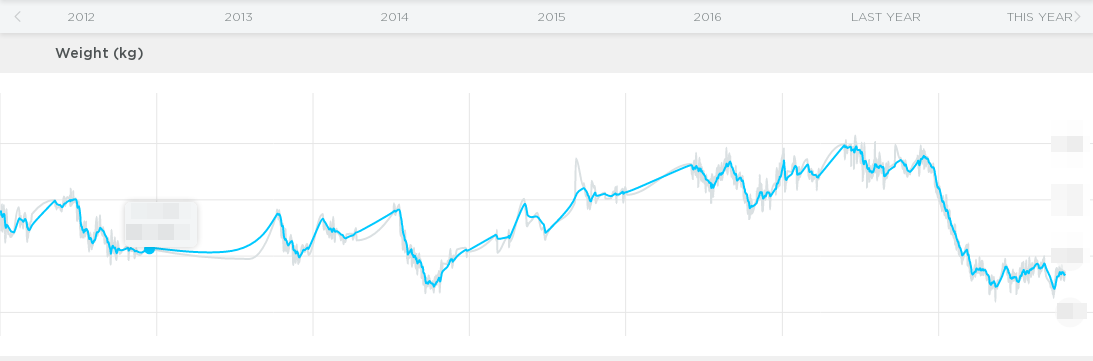
\includegraphics[height=20mm]{images/my-weight.png}
\end{frame}

\section{Introduction}
\begin{frame}
  \frametitle{ }
  \Huge{\bf{Introduction}}
\end{frame}

\section{Today's Goal}
\begin{frame}
  \frametitle{Today's Goal}
  \begin{itemize}
    \item Development ways/tools in OpenStack/OSS communities
    \item Essense of OSS development, it's fun
  \end{itemize}
\end{frame}

\section{Open Source Communities?}
\begin{frame}
  \frametitle{Open Source Communities?}
  There are a lot styles. All OSS projects are different.\\
  Examples: Led by
  \begin{itemize}
    \item Individual (so many, you can find a lot on github)
    \item One company (openSUSE, Ansible, Elastic Search, ..)
    \item Foundation (OpenStack, Kubernetes, Linux kernel, ..)
  \end{itemize}
  Let's take a look at the OpenStack community as an example.
\end{frame}

\section{OpenStack community as an example}
\begin{frame}
  \frametitle{ }
  \Huge{\bf{OpenStack community as an example}}
\end{frame}

\section{What is the OpenStack?}
\begin{frame}
  \frametitle{What is the ``OpenStack''?}
  \begin{itemize}
    \item Written in Python, Open Source Cloud Operation System: Apache License 2.0
    \item One of the top three active OSS communities
    \item There are a lot of `OpenStack' projects: \href{http://governance.openstack.org/reference/projects/index.html}{63 projects(2019-10-05)}
    \item Released every 6 month: Latest version is called `Train'
    \item Users: \scriptsize{AT\&T, AA, BBVA, Bloomberg, CERN,
      China Mobile, Gap, VEXXHOST,
      Volkswagen, WALMART, etc.. \url{https://www.openstack.org/user-stories/}}
  \end{itemize}
  \begin{center}
    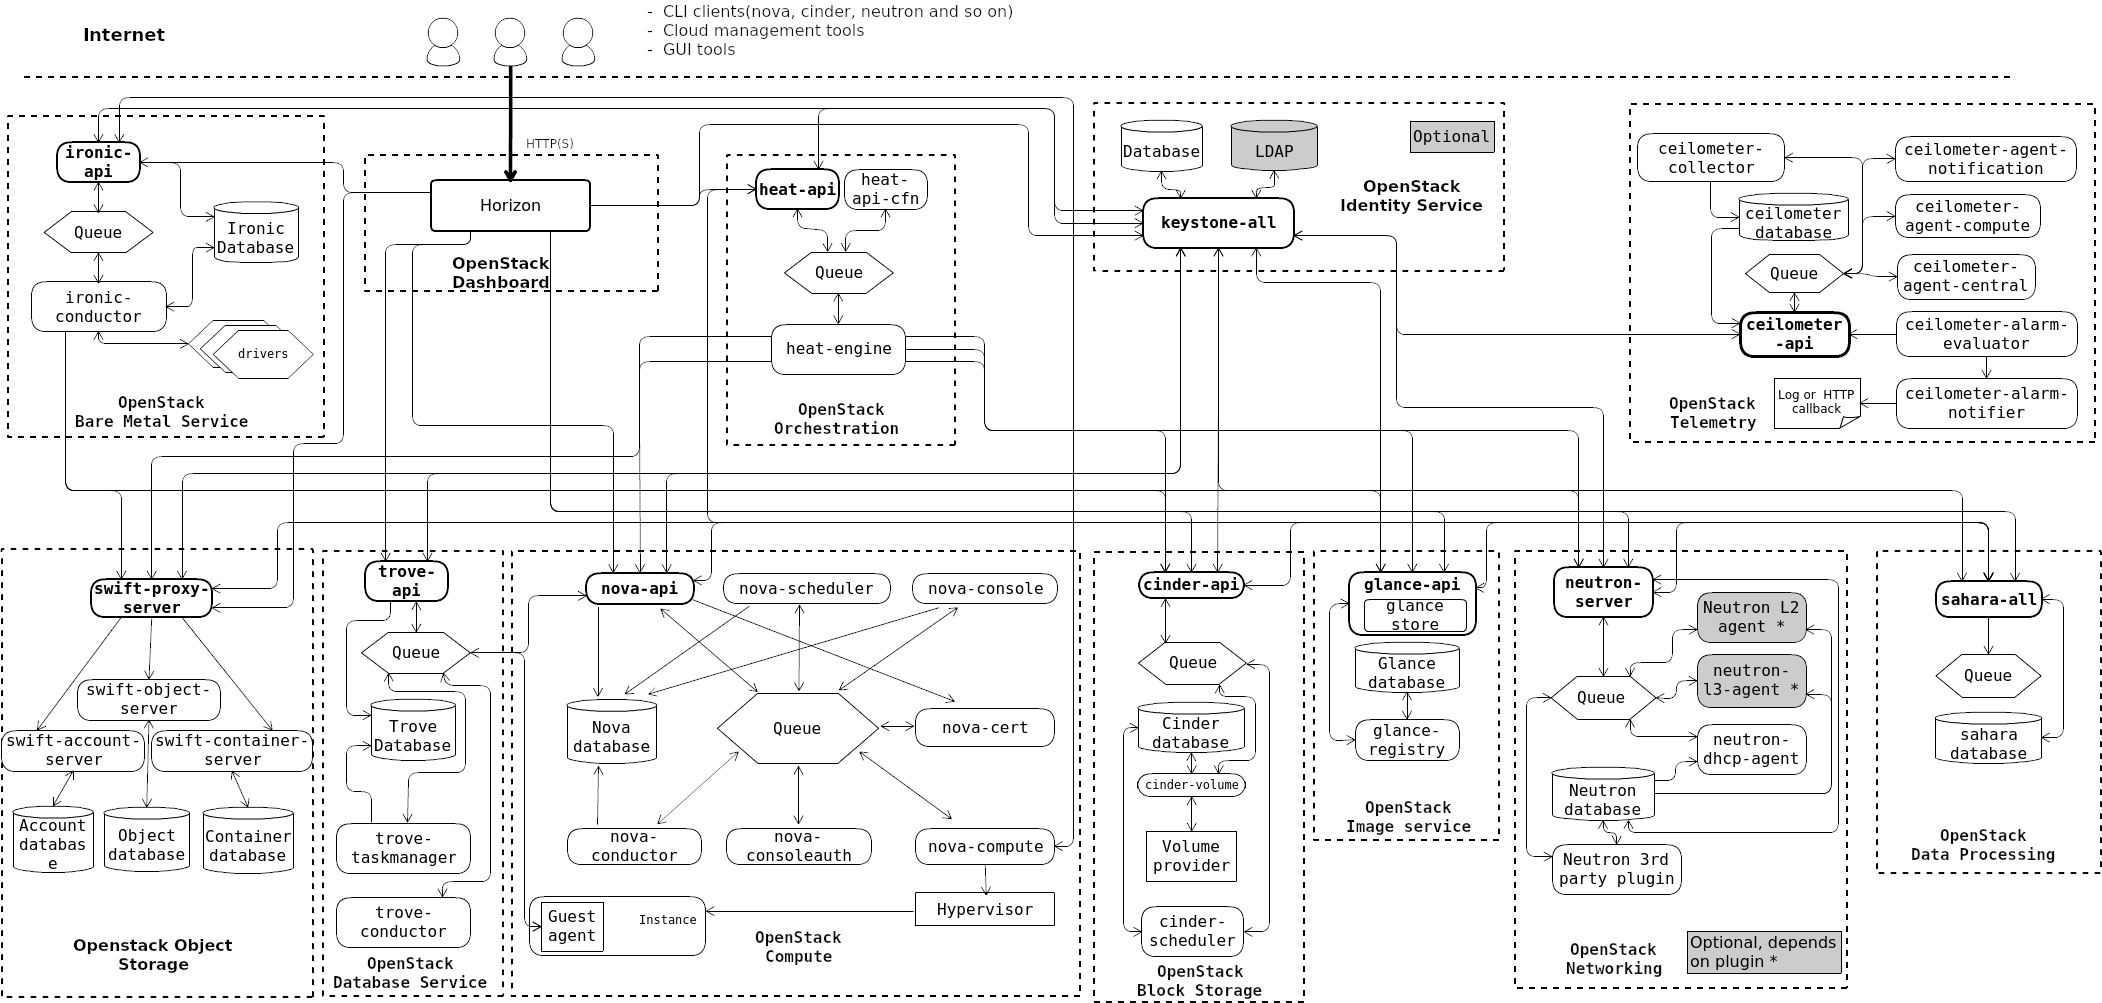
\includegraphics[width=0.7\textwidth]{images/openstack-arch-kilo-logical-v1.png}
  \end{center}
\end{frame}

\section{Workflow of OpenStack development}
\begin{frame}
  \frametitle{Development Workflow in OpenStack}
  \url{https://docs.openstack.org/infra/manual/developers.html}
  \begin{columns}[T]
    \begin{column}{0.5\textwidth}
      \begin{enumerate}
        \item Submit a story to StoryBoard \& discuss (Option)
        \item Make a patch and submit it to Gerrit
        \item Automated testing by Zuul
        \item Review it on Gerrit
        \item Automated testing by Zuul, and merge
      \end{enumerate}
    \end{column}
    \begin{column}{0.4\textwidth}
      \centering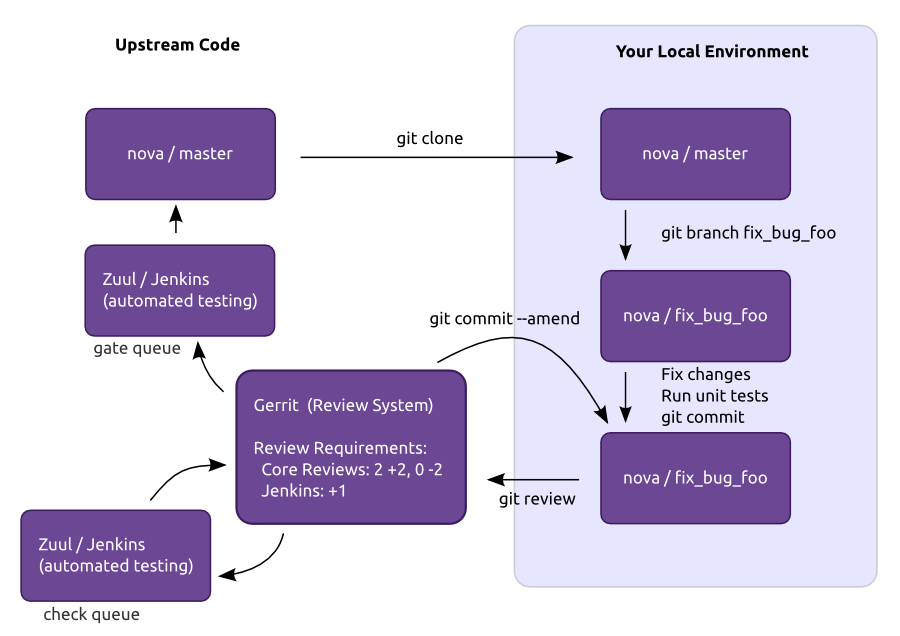
\includegraphics[height=45mm]{images/code_review.png}
    \end{column}
  \end{columns}
\end{frame}

\section{Communication tools}
\begin{frame}
  \frametitle{Tools}
  \begin{itemize}
    \item IRC on Freenode: \#openstack-*(dev,nova,glance,qa,..) \url{https://freenode.net/}
    \item Mailing List: \url{http://lists.openstack.org/}
    \item StoryBoard: \url{https://storyboard.openstack.org/}
    \item Launchpad: \url{https://launchpad.net}
    \item Gerrit: \url{https://review.opendev.org/}
    \item Gitea: \url{https://opendev.org/openstack/}
    \item Zuul: \url{https://zuul.openstack.org}
    \item OpenStack-Health: \url{http://status.openstack.org/openstack-health/}
  \end{itemize}
  \centering
  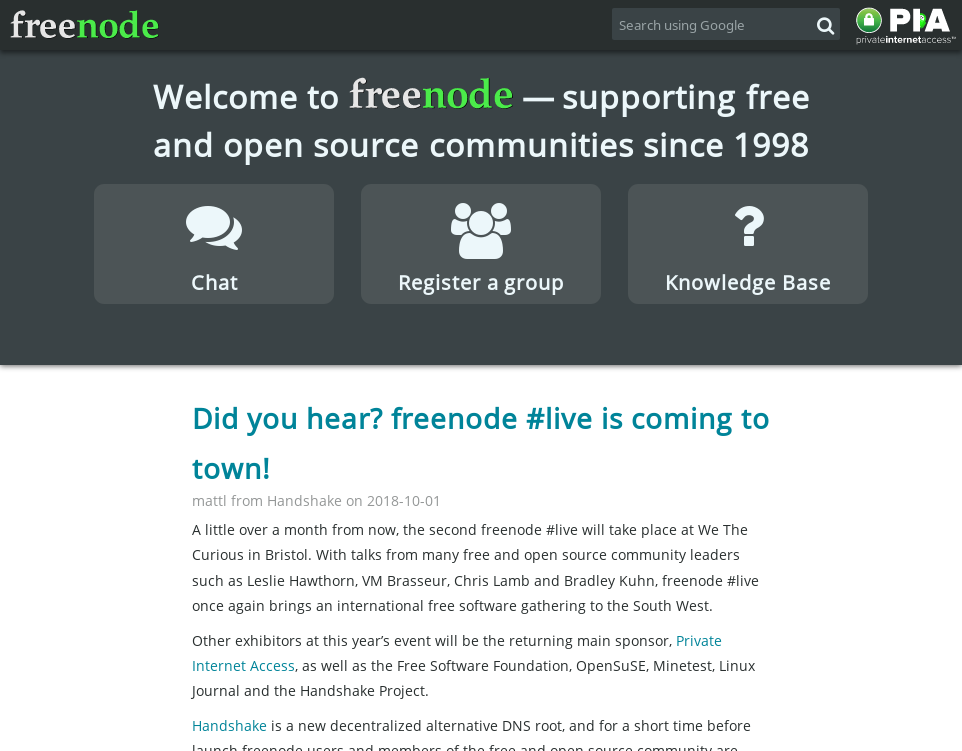
\includegraphics[height=35mm]{images/freenode.png}
  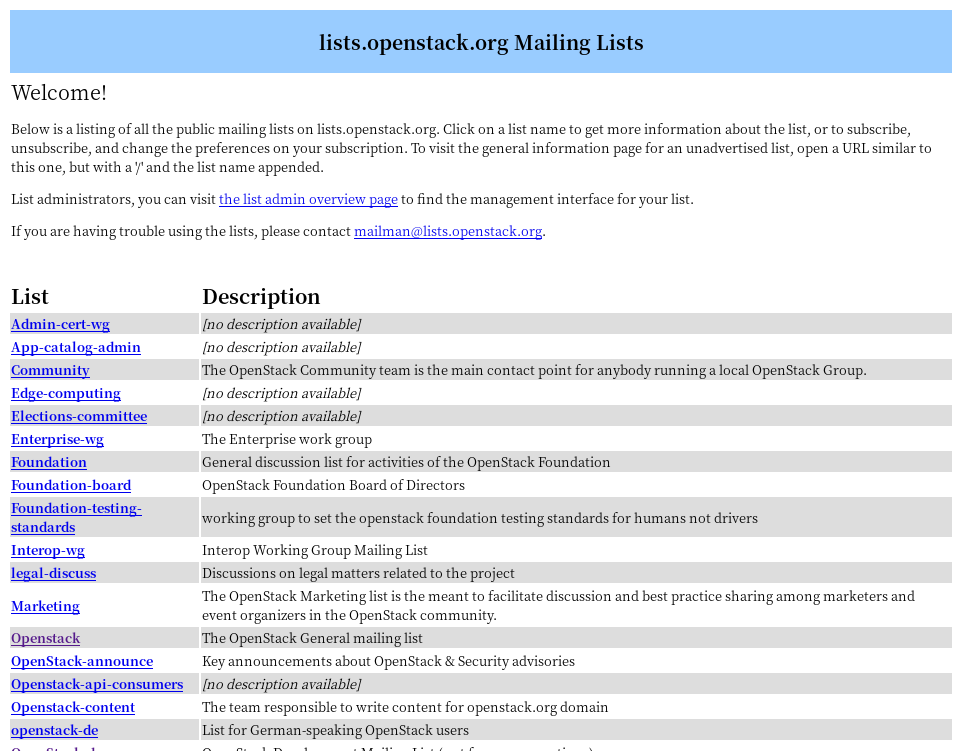
\includegraphics[height=35mm]{images/openstack-ml.png}
  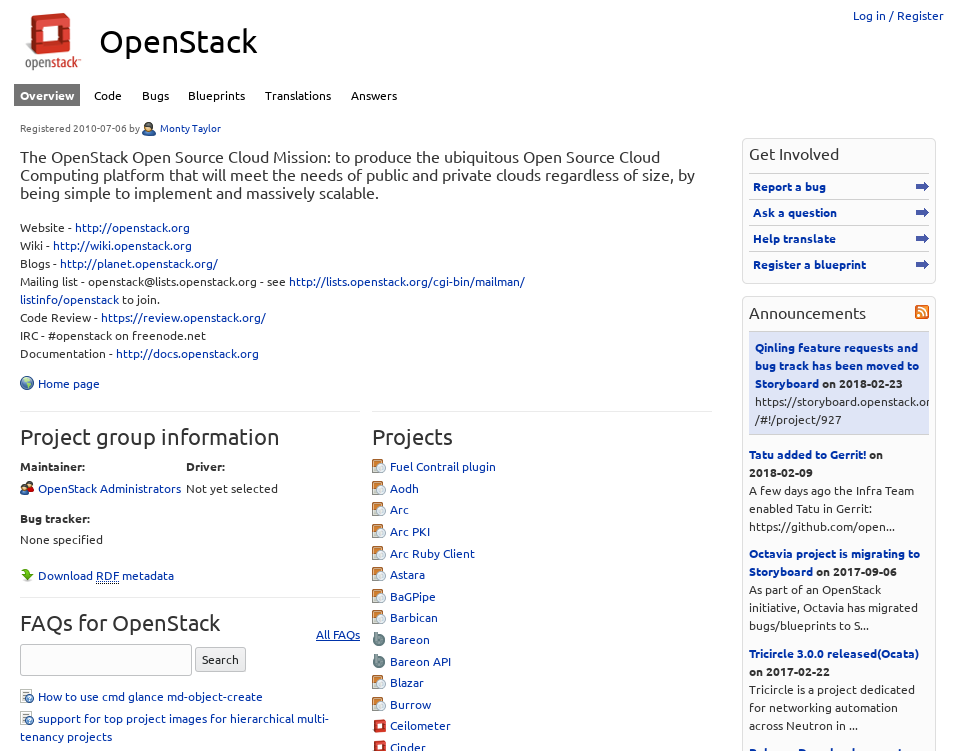
\includegraphics[height=35mm]{images/openstack-in-launchpad.png}
\end{frame}

\begin{frame}
  \frametitle{Project management by StoryBoard - What's ``StoryBoard''}
  \begin{itemize}
    \item Story management tool developed by the OpenStack community
    \item Built from scratch, \url{https://opendev.org/opendev/storyboard/}
    \item Archtecture: {Frontend: JS/Angular, Backend: Python/Pecan}
    \item 100\% open source (Apache2.0)
  \end{itemize}
  \centering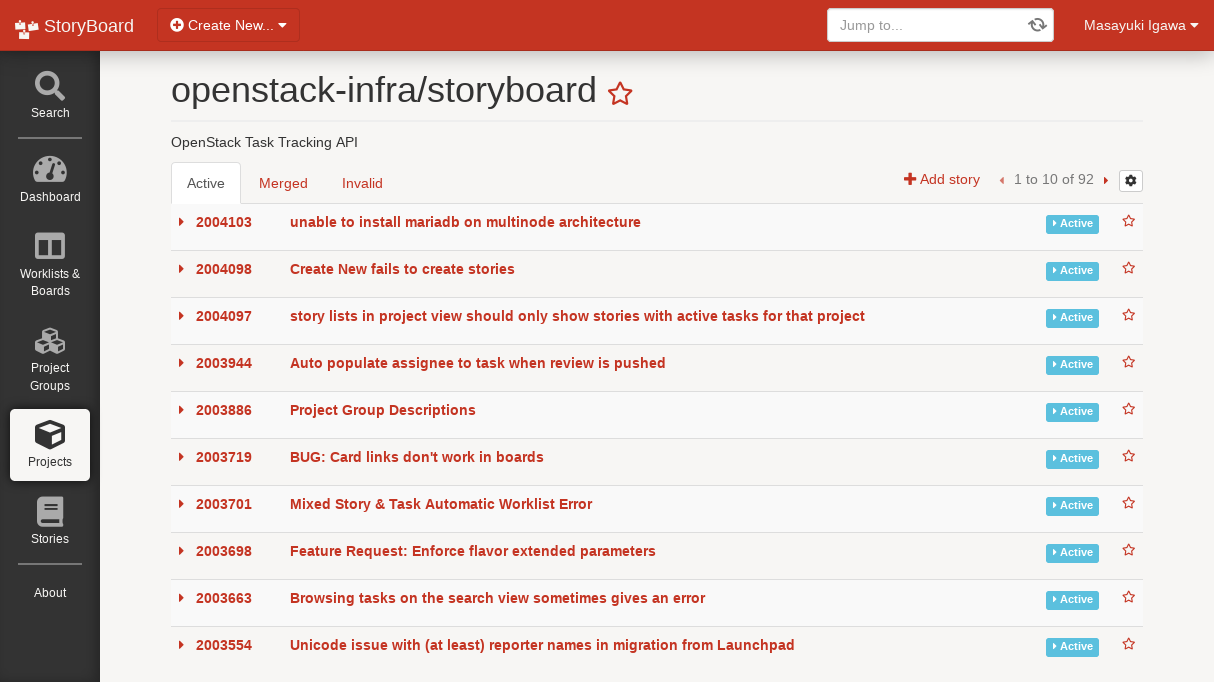
\includegraphics[scale=0.2]{images/storyboard.png}
\end{frame}

\begin{frame}
  \frametitle{Gerrit review system - What's ``Gerrit''}
  \begin{itemize}
    \item Android development community is using it
    \item Java, 100\% open source, \url{https://www.gerritcodereview.com}
    \item Not Pull Request, submit a patch and merge it into a central repo
    \item A terminal client exists > Gertty: \url{https://gertty.readthedocs.io/}
  \end{itemize}
  \centering
  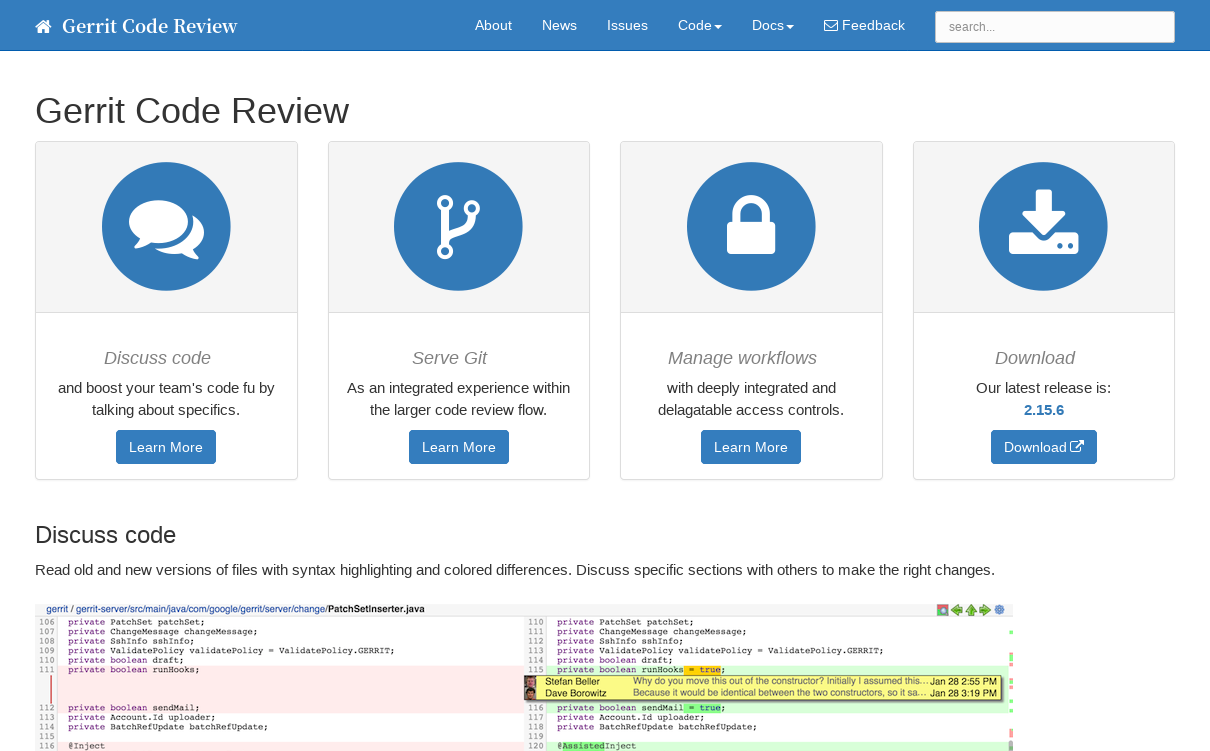
\includegraphics[height=40mm]{images/gerritcodereview-com.png}
  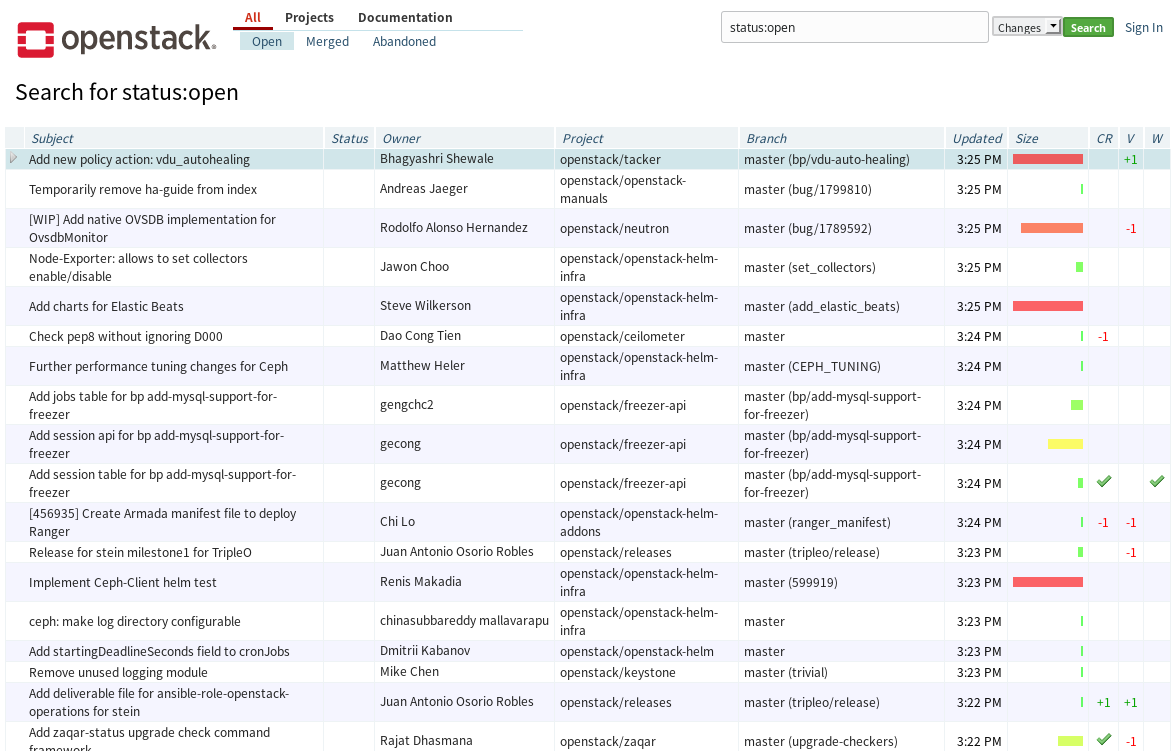
\includegraphics[height=40mm]{images/review-openstack-org.png}
\end{frame}

\begin{frame}
  \frametitle{FYI: Gertty - Gerrit in TTY }
  \begin{itemize}
    \item Terminal client
    \item \url{https://gertty.readthedocs.io/}
    \item Demo
  \end{itemize}
  \centering
  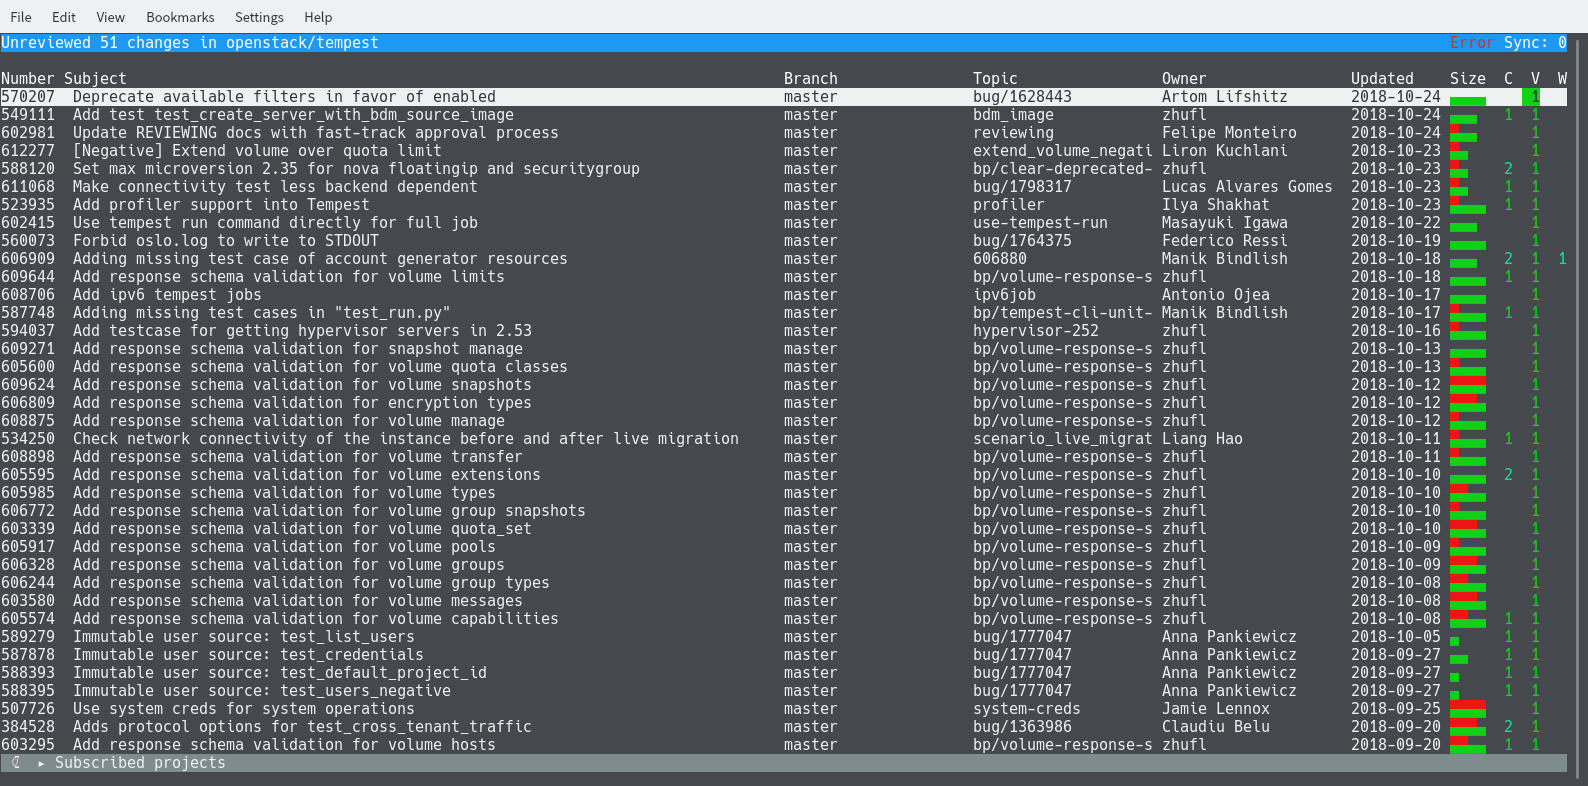
\includegraphics[height=60mm]{images/gertty.png}
\end{frame}

\begin{frame}
  \frametitle{Gitea - Git with a cup of tea}
  \begin{itemize}
    \item A painless self-hosted Git service
    \item Golang, MIT license
    \item \url{https://gitea.io}
  \end{itemize}
  \centering
  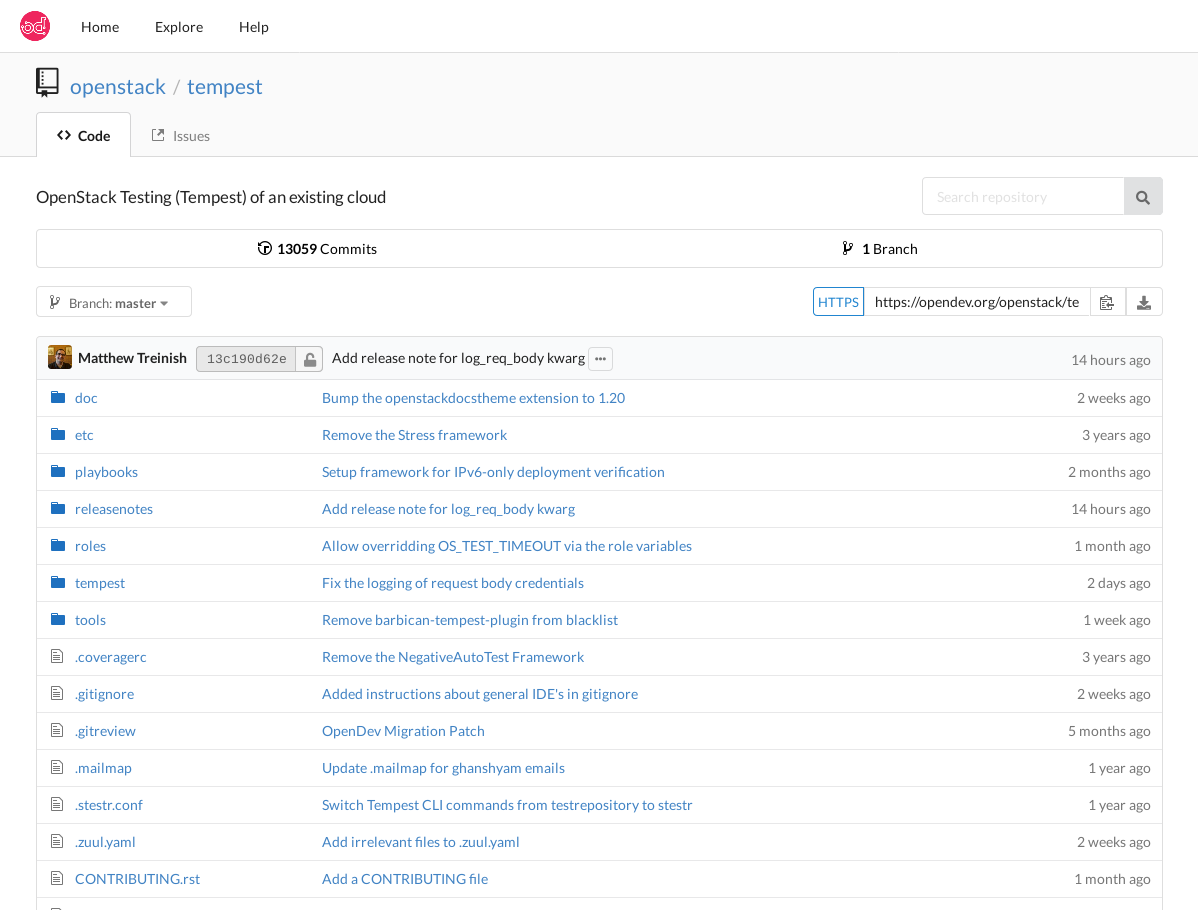
\includegraphics[width=65mm]{images/gitea-tempest.png}
  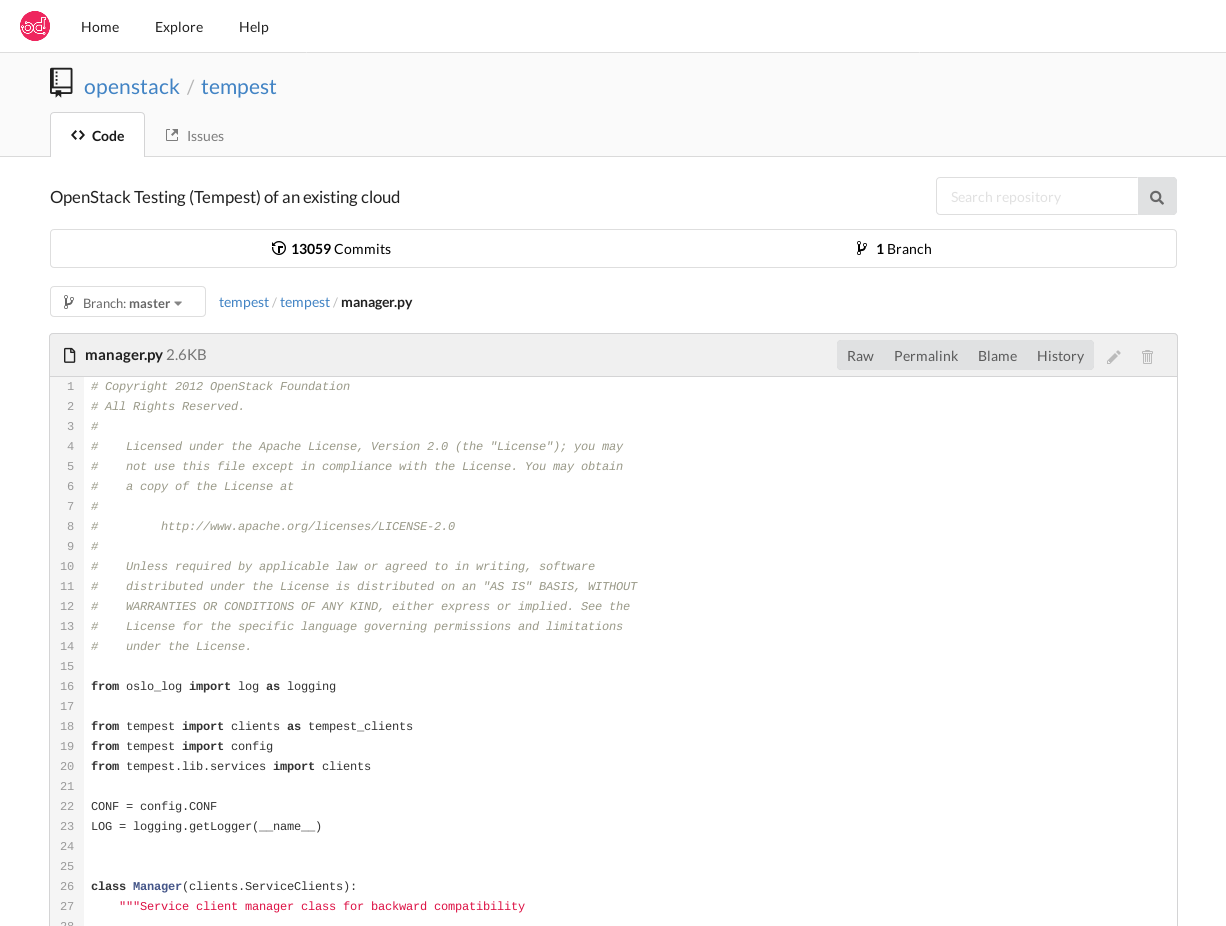
\includegraphics[width=65mm]{images/gitea-tempest-manager.png}
\end{frame}

\begin{frame}
  \frametitle{Continuous Integration by Zuul - What's ``Zuul''}
  \begin{itemize}
    \item \url{https://zuul-ci.org/}
    \item Set a gate by automated testing - Stop Merging Broken Code    
    \item CI/CD powered by Ansible
    \item Cross-Project Dependencies can be tested
  \end{itemize}
  \centering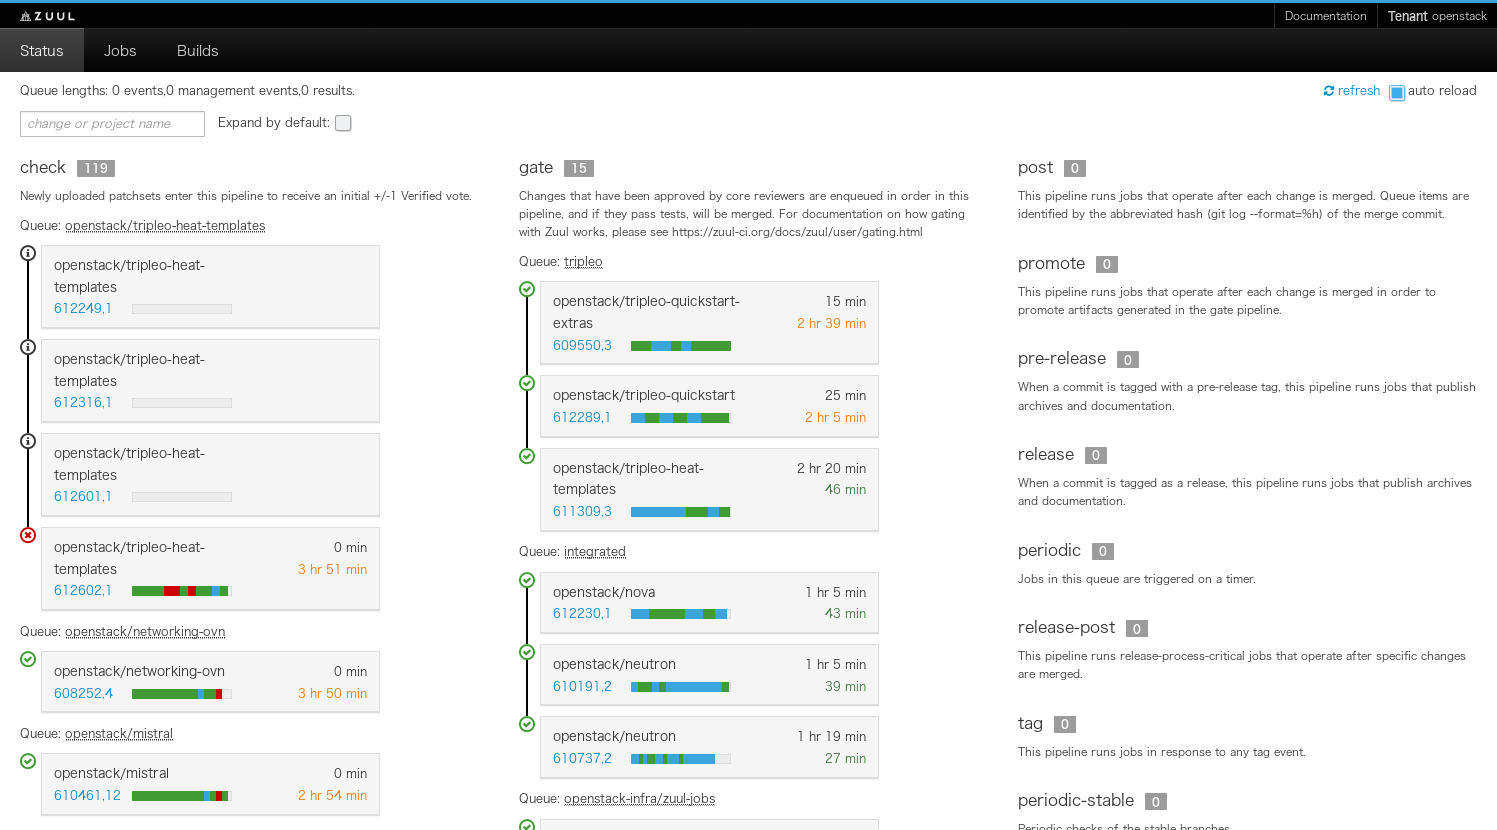
\includegraphics[scale=0.2]{images/zuul-status.png}
\end{frame}

\begin{frame}
  \frametitle{Gate Health check by OpenStack Health}
  \begin{itemize}
    \item Story management tool developed by the OpenStack community
    \item Built from scratch, \url{https://opendev.org/openstack/openstack-health/}
    \item Archtecture: {Frontend: JS/Angular, Backend: Python/Flask}
    \item 100\% open source (Apache2.0)
  \end{itemize}
  \centering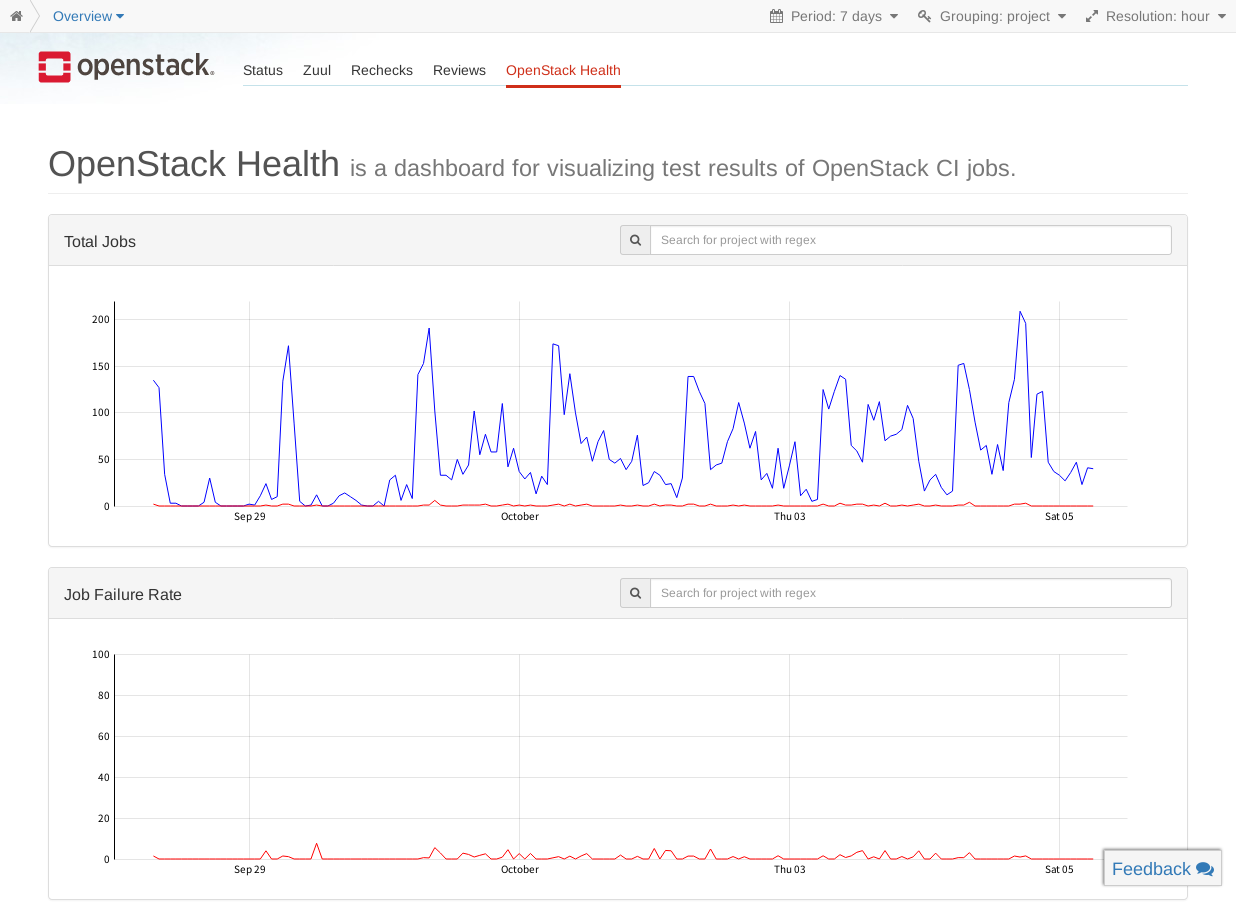
\includegraphics[width=60mm]{images/openstack-health1.png}
  \centering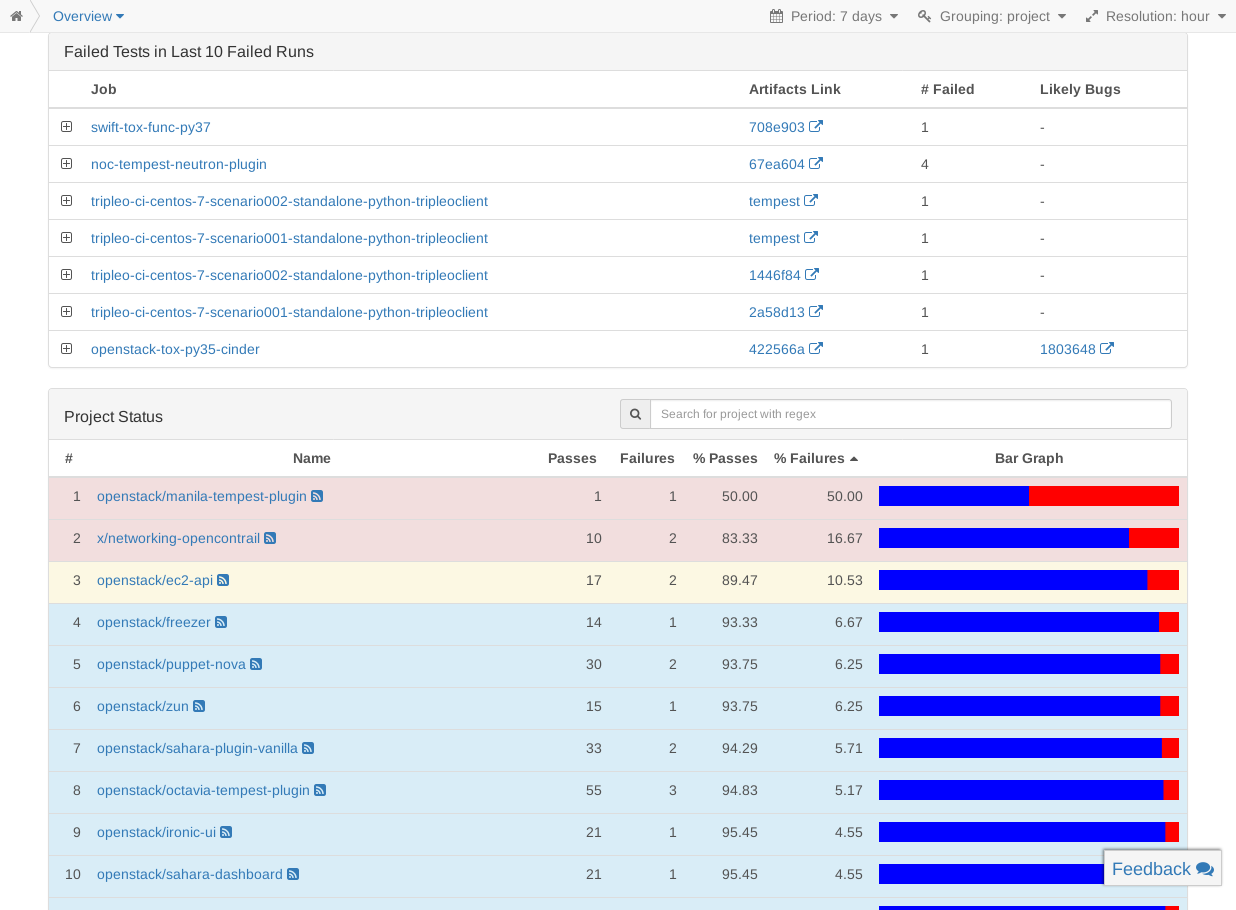
\includegraphics[width=60mm]{images/openstack-health2.png}
\end{frame}

\section{Inside Story}
\begin{frame}
  \frametitle{Inside Story}
  \begin{enumerate}
    \item Very long time to get merged, why?
    \item Unstable and Slow CI
    \item Communication is important
  \end{enumerate}
\end{frame}

\begin{frame}
  \frametitle{1. Very long time to get merged, why?}
  \begin{itemize}
    \item Project size ≒ Number of stakeholders
    \item Less communication (sending an email isn't a good idea)
    \item Less reviewers (next slide)
    \item Unstable and Slow CI
  \end{itemize}
\end{frame}

\begin{frame}
  \frametitle{1. Less reviewers (cont. Why?)}
  \centering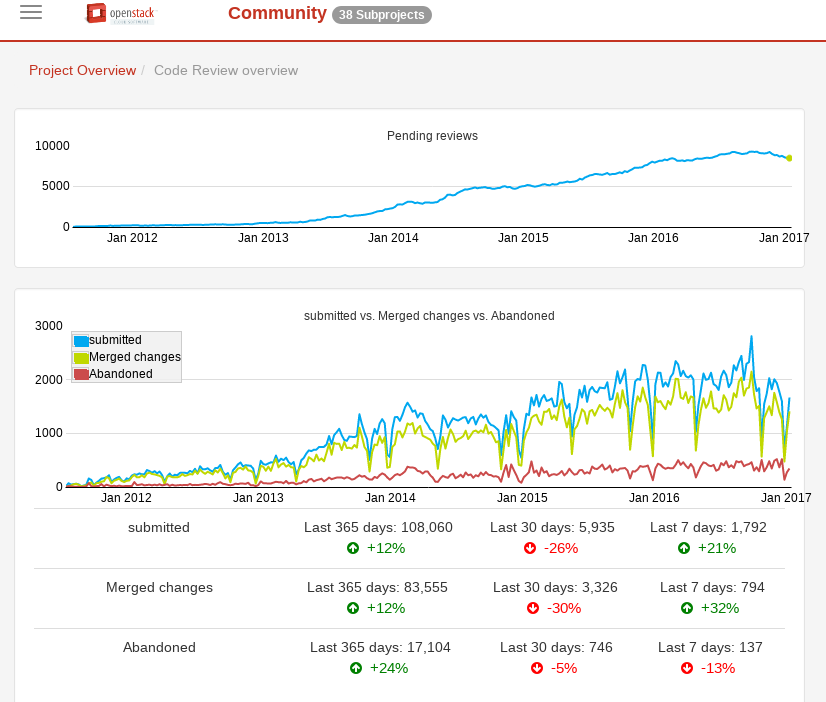
\includegraphics[height=70mm]{images/project-overview.png}
  \url{http://activity.openstack.org/dash/browser/scr.html}
\end{frame}

\begin{frame}
  \frametitle{2. Unstable and Slow CI}
  \begin{itemize}
    \item Easily rot if the code doesn't work in CI
    \item ``CI'' is not perfect
    \item Busy neighbors problem
    \item Rapid fixing is necessary - next slide
  \end{itemize}
\end{frame}

\begin{frame}
  \frametitle{2. Elastic Recheck (cont. Unstable and Slow CI)}
    Correlate a bug to a signature in a log, and detect the bug automatically
  \centering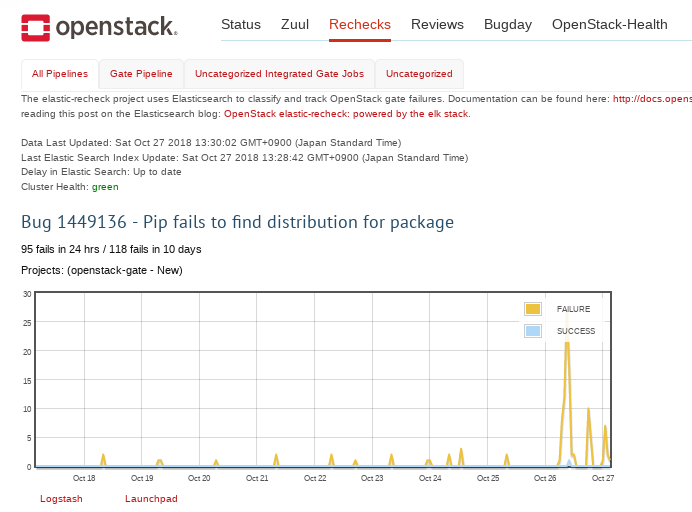
\includegraphics[width=60mm]{images/elastic-recheck.png}
  \centering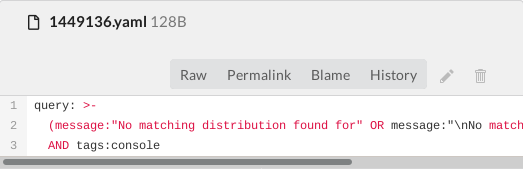
\includegraphics[width=75mm]{images/elastic-recheck-source.png}
  \url{http://status.openstack.org/elastic-recheck/},
  \url{https://opendev.org/opendev/elastic-recheck/src/branch/master/queries/1737039.yaml}
\end{frame}

\begin{frame}
  \frametitle{3. Communication is important (English is hard)}
  \begin{itemize}
    \item Discussion
    \item Find a job (e.g. difficul to get good salary as a programmer basically in Japan)
    \item Fun (Take care of yourself! :)
  \end{itemize}
  \centering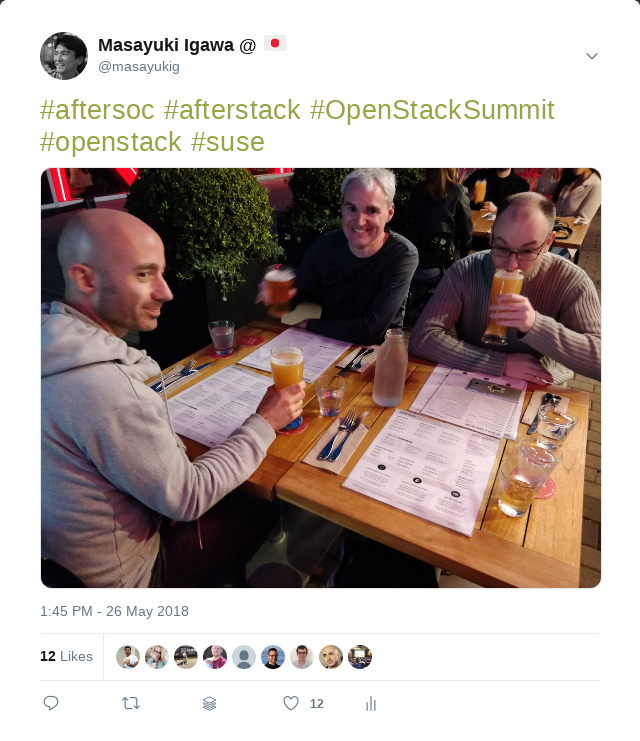
\includegraphics[height=60mm]{images/tweet-suse.png}
  \centering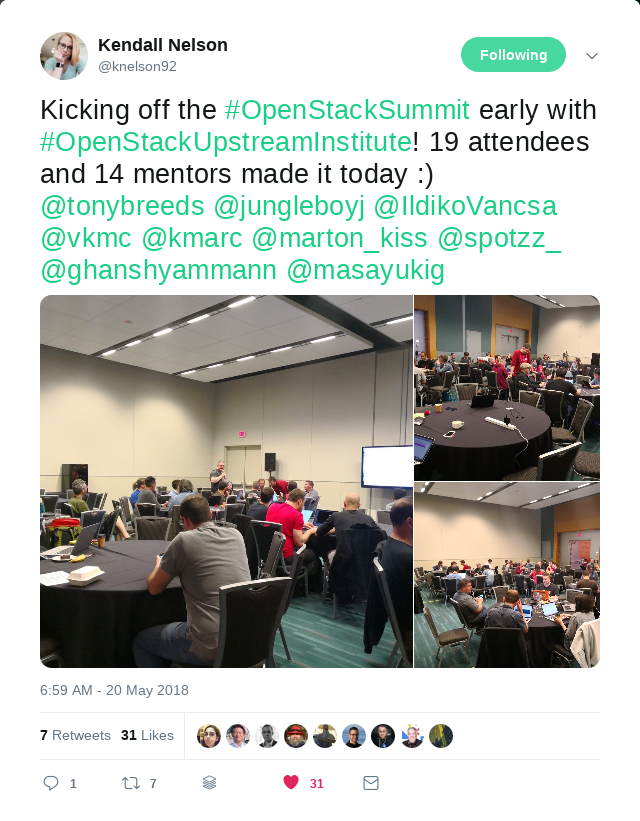
\includegraphics[height=60mm]{images/tweet-oui.png}
\end{frame}

\begin{frame}
  \frametitle{3. English as a second language (cont. Communication is important)}
  \begin{itemize}
    \item We have a document: \url{https://docs.openstack.org/doc-contrib-guide/non-native-english-speakers.html}
    \item Not only language but also culture (For example: Zensho shimasu (善処します))
  \end{itemize}
\end{frame}

\section{How to participate Open Source Community}
\begin{frame}
  \frametitle{ }
  \Huge{\bf{How to participate Open Source Community}}
\end{frame}

\begin{frame}
  \frametitle{How to participate Open Source development}
  \begin{itemize}
    \item Find projects which you are interested in
    \item Find online/offline mentor(s) and friends
    \item Understand culture of communities
    \item Not only code, using/testing, submit bugs/issues, documentation, translation, etc.
    \item As a study, hobby or job?
  \end{itemize}
  \centering
\includegraphics[height=50mm]{images/hacktoberfest.png}
  \url{https://hacktoberfest.digitalocean.com/}
\end{frame}

\section{Conclusion}
\begin{frame}
  \frametitle{Conclusion}
  \begin{itemize}
    \item Gerrit, StoryBoard, Zuul, OSS can be used for non-OSS product
    \item Communication is important, and English too
    \item Development OSS is fun! and tough sometimes. Why not participate in it?
  \end{itemize}
  Appendix
  \begin{itemize}
      \item Slides: \url{https://github.com/masayukig/oss-development-inside-story/blob/master/oss-development-inside-story.pdf}
      \item Contact info: \texttt{masayukig on
        \href{https://freenode.net/}{Freenode},
        \href{https://github.com/masayukig}{GitHub},
        \href{https://twitter.com/masayukig}{Twitter},
        \href{https://www.linkedin.com/in/masayukig/}{LinkedIn}}
      \item StoryBoad: \url{https://docs.openstack.org/infra/system-config/storyboard.html}
      \item Gerrit: \url{https://www.gerritcodereview.com/}
      \item Zuul: \url{https://zuul-ci.org/}
      \item Non-native English speakers in Open Source communities: \url{http://bit.ly/esl-yvr}
  \end{itemize}
\end{frame}

\end{document}
